\section{Experiments}
\label{sec:experiments}

\subsection{Experimental Setup}
\label{sec:exp_setup}

\paragraph{Benchmark.} We evaluate on LIBERO~\cite{liu2023libero}, a simulated tabletop manipulation benchmark with four suites of increasing complexity: \textbf{Object} (10 tasks, visually similar objects), \textbf{Spatial} (10, relative spatial layouts), \textbf{Goal} (10, goal-conditioned manipulation), and \textbf{Long} (10, chained 3--5 step sequences). Each task has 50 demo and 50 evaluation episodes (500 per suite).

\paragraph{Models.} Four VLAs are evaluated in closed-loop control (Table~\ref{tab:model_properties}): $\pi_{0.5}$~\cite{black2025pi05}, X-VLA~\cite{zheng2025xvla}, OpenVLA~\cite{kim2024openvla}, and SmolVLA~\cite{shukor2025smolvla}. Two additional models ($\pi_{0}$, OFT) contribute to the CV diagnostic via offline metrics only.

\paragraph{Protocol.} We prune at $k \in \{0.3, 0.5, 0.7, 0.75, 0.85, 0.9, 0.95\}$ and report mean SR over 500 episodes. Multi-seed results ($\pi_{0.5}$ Long: $n{=}5$; VTR: $n{=}3$) report mean $\pm$ s.d.\ with per-seed breakdowns in the appendix.

\begin{figure}[t]
\centering
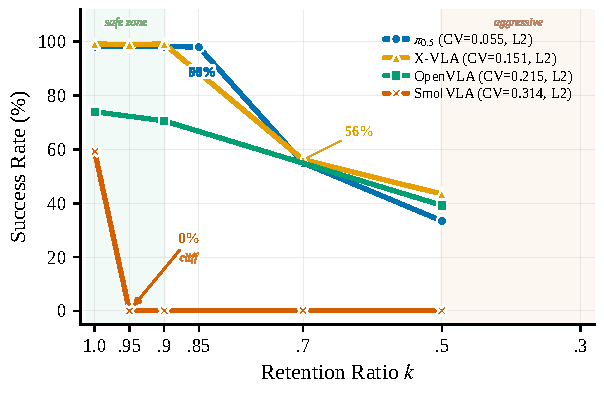
\includegraphics[width=0.75\linewidth]{figures/paper/fig_pruning_overview.pdf}
\caption{Pruning degradation on LIBERO-Object (L2 norm scoring). $\pi_{0.5}$ maintains ${\geq}$98\% through $k{=}0.85$, OpenVLA degrades linearly, X-VLA cliffs at $k{=}0.7$, SmolVLA collapses to 0\% at $k{=}0.95$.}
\label{fig:pruning_overview}
\end{figure}

\subsection{Two-Axis Framework Overview}
\label{sec:two_axis}

Three qualitatively distinct response patterns emerge across the connector spectrum (Table~\ref{tab:main_results}; Figure~\ref{fig:pruning_overview}); a fourth (OpenVLA, MLP connector) is detailed in Appendix Table~\ref{tab:full_results}.

\textbf{$\pi_{0.5}$ (linear, CV$\,{=}\,$0.055).} Low-CV models are \emph{uniformly critical}: which tokens are removed matters more than how many. On Object, L2 maintains ${\geq}$98.0\% through $k{=}0.85$ (Appendix Table~\ref{tab:full_results}), while random at $k{=}0.9$ collapses to 9.0\%, an 89\,pp (percentage points) method gap from identical removal fractions.

\textbf{X-VLA (BART encoder, CV$\,{=}\,$0.151).} Method-insensitive but task-sensitive: at $k{=}0.9$ on Object, L2 and random differ by 1.4\,pp, yet the same model drops 28.2\,pp on Goal. Removing 3 of 50 tokens ($k{=}0.95$) halves Long SR regardless of method.

\textbf{OpenVLA (MLP, CV$\,{=}\,$0.215).} OpenVLA exhibits scoring crossover: L2 outperforms random on Object but the ranking inverts on Spatial and Goal at $k{=}0.9$ (Appendix Table~\ref{tab:full_results}; Appendix~\ref{app:extended_discussion}).

\textbf{SmolVLA (pixel-shuffle, CV$\,{=}\,$0.314).} Removing 7 of 128 tokens ($k{=}0.95$) collapses SR to ${\leq}$6.6\% across all suites and methods, a catastrophic cliff detailed in Section~\ref{sec:pixel_shuffle}.

\begin{table*}[t]
\centering
\small
\caption{Closed-loop SR (\%) on LIBERO under L2 norm (L2) and random (R) pruning. $\pi_{0.5}$ Long: five-seed mean ($n{=}5$). Full results including OpenVLA in Appendix Table~\ref{tab:full_results}.}
\label{tab:main_results}
\begin{tabular}{llcccc}
\toprule
Model & Suite & Baseline & $k{=}0.95$ (L2 / R) & $k{=}0.9$ (L2 / R) & $k{=}0.5$ (L2 / R) \\
\midrule
\multirow{4}{*}{$\pi_{0.5}$}
& Object  & \textbf{98.2} & 98.2 / 74.0 & \textbf{98.2} / 9.0 & 33.4 / 69.4 \\
& Spatial & \textbf{97.2} & \textbf{97.8} / 76.4 & 95.0 / 54.6 & 55.6 / 71.6 \\
& Goal    & \textbf{96.4} & 89.4 / 84.0 & 90.6 / 62.2 & 59.2 / 73.6 \\
& Long    & \textbf{91.6} & 86.8 / 61.2 & 80.4 / 33.6 & 51.7 / 50.4 \\
\midrule
\multirow{4}{*}{X-VLA}
& Object  & \textbf{99.2} & 99.0 / 98.8 & 99.2 / 97.8 & 43.4 / 70.6 \\
& Spatial & \textbf{93.0} & 71.6 / 70.2 & 78.8 / 77.8 & 58.8 / 71.4 \\
& Goal    & \textbf{98.4} & 53.8 / 54.0 & 70.2 / 70.6 & 59.0 / 67.2 \\
& Long    & \textbf{94.0} & 47.0 / 48.2 & 27.5 / 29.6 & 45.0 / 61.6 \\
\midrule
\multirow{4}{*}{SmolVLA}
& Object  & \textbf{59.2} & 0.0 / 0.0 & 0.0 / 0.0 & 0.0 / 0.0 \\
& Spatial & \textbf{44.6} & 6.6 / 4.2 & 0.0 / 0.0 & 0.0 / 0.0 \\
& Goal    & \textbf{60.8} & 3.4 / 4.2 & 0.0 / 0.0 & 0.0 / 0.0 \\
& Long    & \textbf{36.6} & 0.0 / 0.0 & 0.0 / 0.0 & 0.0 / 0.0 \\
\bottomrule
\end{tabular}
\end{table*}

\begin{figure*}[t]
\centering
\begin{subfigure}[t]{0.49\textwidth}
\centering
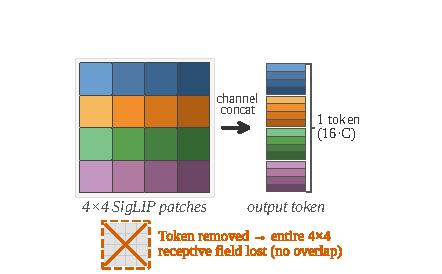
\includegraphics[width=\linewidth]{figures/paper/fig_pixel_shuffle.pdf}
\caption{}
\label{fig:pixel_shuffle}
\end{subfigure}\hfill%
\begin{subfigure}[t]{0.49\textwidth}
\centering
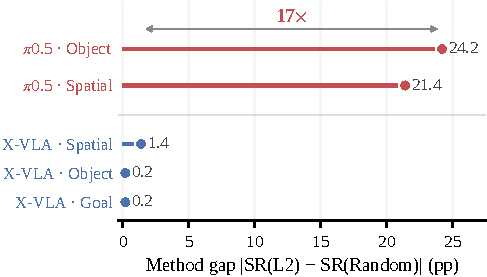
\includegraphics[width=\linewidth]{figures/paper/fig_method_gap.pdf}
\caption{}
\label{fig:method_gap}
\end{subfigure}
\caption{(a)~Pixel-shuffle $4{\times}4$ entanglement: each 16-patch block forms one token; removing any eliminates a non-overlapping receptive field with no redundancy. (b)~Method gap $|\text{SR(L2)} - \text{SR(Random)}|$ at $k{=}0.95$: $\pi_{0.5}$'s Object gap (24.2\,pp) exceeds X-VLA's maximum (1.4\,pp) by $17{\times}$ (single seed except $\pi_{0.5}$ Long, $n{=}5$).}
\label{fig:entanglement_and_gap}
\end{figure*}

\subsection{Pixel-Shuffle Entanglement}
\label{sec:pixel_shuffle}

SmolVLA's pixel-shuffle $4{\times}4$ folding concatenates 16 patches per token (Figure~\ref{fig:pixel_shuffle}), creating non-overlapping receptive fields. Removing any token eliminates an entire spatial block, collapsing SR to ${\leq}$6.6\% at $k{=}0.95$ across all suites and methods (verified on two checkpoints; Appendix~\ref{app:smolvla_ablation}). X-VLA's BART encoder is also entangling, yet far more robust: its 12-layer self-attention redistributes information across tokens, creating inter-token redundancy that buffers against removal. Pixel-shuffle performs a fixed deterministic fold with no learned information sharing; each output token's receptive field is disjoint, leaving zero redundancy for pruning to exploit.

\begin{figure}[t]
\centering
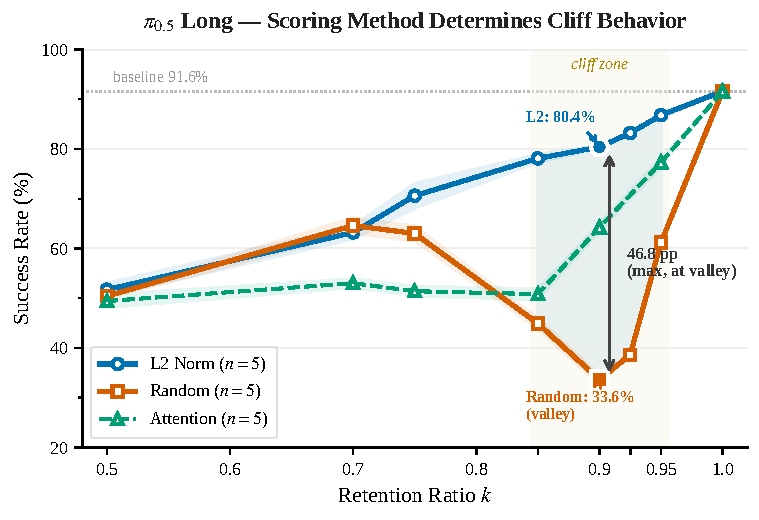
\includegraphics[width=0.75\linewidth]{figures/paper/fig_cliff_highlight.pdf}
\caption{Scoring method cliff behavior on $\pi_{0.5}$ Long ($n{=}5$, mean $\pm$ s.d.). L2 degrades monotonically; attention cliffs at $k{=}0.85$; random V-shapes with collapse at $k{=}0.9$.}
\label{fig:cliff_highlight}
\end{figure}

\subsection{Position Disruption vs.\ Information Loss}
\label{sec:zeromask}

$\pi_{0.5}$'s random pruning at $k{=}0.9$ collapses to 9.0\% on Object despite removing only 10\% of tokens. We compare hard pruning (removes tokens, re-indexes positions) with zero-masking (zeros embeddings, preserves positions): zero-masking preserves 98.0\% SR while hard pruning collapses to 9.0\%. On $\pi_{0.5}$, the 89\,pp gap is entirely attributable to position disruption: its linear connector tolerates complete signal destruction but not index shifts. This ablation targets $\pi_{0.5}$ because its Rotary Position Embedding (RoPE)-based position encoding is most susceptible to re-indexing; other connectors use different positional mechanisms.

This has practical implications: for position-sensitive architectures, any compression that alters the sequence length will disrupt positional encodings. Strategies for such models must either preserve the original length (e.g., zero-masking) or include position-aware mechanisms that compensate for index shifts.

\subsection{Scoring Method Sensitivity and CV Diagnostic}
\label{sec:cv_sensitivity}

CV predicts where scoring method choice becomes critical (Figure~\ref{fig:method_gap}). $\pi_{0.5}$'s Object gap at $k{=}0.95$ reaches 24.2\,pp, exceeding X-VLA's maximum (1.4\,pp) by $17{\times}$. At $k{=}0.5$, the importance margin on Object is $\Delta{=}{-}36.0$\,pp ($\pi_{0.5}$) and ${-}27.2$\,pp (X-VLA): L2 scoring clusters spatially correlated tokens at the cost of spatial diversity.

\textbf{Architecture-dependent scoring.} The optimal scoring method depends on the connector (Table~\ref{tab:attention_pruning}). On X-VLA at $k{=}0.5$, attention recovers ${\geq}$92.8\% while L2 falls 8--27\,pp below random; on $\pi_{0.5}$, attention is catastrophically harmful on Object ($-$31.6\,pp). On Long, attention cliffs $-$26.5\,pp from $k{=}0.95$ to $k{=}0.85$, then plateaus (Figure~\ref{fig:cliff_highlight}).

\textbf{Inverted-U importance margin.} On $\pi_{0.5}$ Long, $\Delta$ peaks at $k{=}0.9$ ($+$46.8\,pp), diminishes at $k{=}0.95$ ($+$25.6\,pp) where both methods suffice, and converges at $k{=}0.5$ ($+$1.3\,pp) where both are inadequate. Near $k{\approx}0.7$, the ranking inverts as L2 concentrates tokens spatially at the cost of coverage (Figure~\ref{fig:cliff_highlight}; Appendix Figure~\ref{fig:margin_profile}).

\textbf{Importance margin gradient.} L2's advantage shrinks with task complexity on $\pi_{0.5}$ at $k{=}0.85$: Object $\Delta{=}+$92.4\,pp $>$ Goal $+$35.2\,pp $>$ Long $+$33.2\,pp (Appendix Table~\ref{tab:full_results}).

\subsection{VTR Recovery}
\label{sec:vtr_recovery}

\begin{table}[t]
\centering
\small
\caption{VTR on SmolVLA (LIBERO-Object). Hard pruning collapses to 0\%; VTR exceeds the unpruned baseline at up to 87.5\% compression. Baseline (44.8\%) is our Low-Rank Adaptation (LoRA) reproduction; official checkpoint achieves 59.2\% (Table~\ref{tab:main_results}).}
\label{tab:vtr_main}
\begin{tabular}{lccr}
\toprule
Configuration & $M$ & Compress.\ & SR (\%) \\
\midrule
\textit{Baseline (unpruned)} & 128 & 0\% & 44.8 \\
\textit{Hard pruning (any)} & -- & 5--50\% & 0.0 \\
\midrule
Cross-attn VTR & 32 & 75\% & 60.1 $\pm$ 1.3 \\
Cross-attn VTR & 16 & 87.5\% & 56.9 $\pm$ 1.3 \\
MLP adapter & 32 & 75\% & 63.4 $\pm$ 2.6 \\
\bottomrule
\end{tabular}
\end{table}

VTR uses $M$ learned queries cross-attending over all 128 source tokens (${\sim}$22M parameters, $<$5\% of SmolVLA). At 75\% compression, VTR achieves 60.1 $\pm$ 1.3\% SR ($M{=}32$, $n{=}3$; Table~\ref{tab:vtr_main}), exceeding the unpruned LoRA baseline (44.8\%) by 15.3\,pp. An extended training control rules out additional optimization as the source ($p > 0.9$; Appendix~\ref{app:smart_compress_details}). A parameter-matched MLP adapter achieves 63.4 $\pm$ 2.6\% ($p{=}0.15$), indicating the benefit stems from re-encoding rather than the specific cross-attention mechanism. This suggests the key ingredient is providing a learnable interface between the entangled connector output and the LLM input, allowing the model to reconstruct a compressed representation that respects the LLM's positional expectations.

Performance scales gracefully with compression: reducing $M$ from 32 to 16 (87.5\% compression) costs only 3.2\,pp, while still exceeding the unpruned baseline by 12.1\,pp. Cross-suite generalization confirms the learned compression transfers: Spatial recovers to 53.2\% and Goal to 56.4\%, both from 0.0\% under hard pruning, without suite-specific training. For $\pi_{0.5}$, $k{=}0.9$ with L2 scoring cuts attention FLOPs by ${\sim}$16\% while preserving full SR, requiring no additional parameters.
